%\documentclass[tikz, border=5pt]{standalone}
\begin{document}
	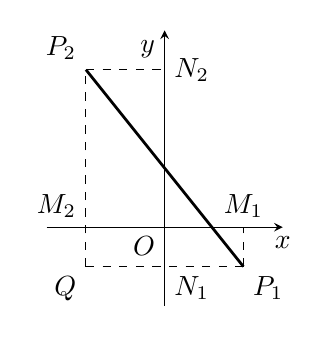
\begin{tikzpicture}[>=stealth, scale=0.5] % 箭头样式为stealth,
		
		% 绘制坐标轴
		\draw[->] (-3,0) -- (3,0) node[below] {$x$}; % x轴(带箭头和标签)
		\draw[->] (0,-2) -- (0,5) node[below left] {$y$}; % y轴(带箭头和标签)
		\node at (0,0) [below left] {$O$};           % 原点O的标签
		
		% 定义各关键点坐标
		\coordinate (P1) at (2,-1);  % 点P₁
		\coordinate (P2) at (-2,4); % 点P₂
		\coordinate (N1) at (0,-1); % 点N₁
		\coordinate (N2) at (0,4);  % 点N₂
		\coordinate (M1) at (2,0);  % 点M₁
		\coordinate (M2) at (-2,0); % 点M₂
		\coordinate (Q)  at (-2,-1);% 点Q
		
		% 绘制连接P₁和P₂的直线
		\draw[line width=1pt] (P1) -- (P2);
		
		% 绘制虚线辅助线(矩形的边)
		\draw[dashed] (P2) -- (N2); % P₂到y轴的虚线
		\draw[dashed] (Q) -- (P2);  % Q到P₂的虚线
		\draw[dashed] (Q) -- (P1);  % Q到P₁的虚线
		\draw[dashed] (P1) -- (M1); % P₁到x轴的虚线
		
		% 标记各点的标签
		\node at (P1) [below right]  {$P_1$};
		\node at (P2) [above left]      {$P_2$};
		\node at (N1) [below right] {$N_1$};
		\node at (N2) [right]             {$N_2$};
		\node at (M1) [above]          {$M_1$};
		\node at (M2) [above left] {$M_2$};
		\node at (Q)  [below left]   {$Q$};
		
	\end{tikzpicture}
\end{document}
